\section{Traction Control Mode Architecture}
\label{s:TCMA}
Figure \ref{fig:Traction_Control_Mode_Block_Diagram} is a block diagram of the higher level architecture of the traction control mode and each of its components discussed in sections \ref{s:DTKF}, \ref{s:MME}, and \ref{s:TC}. In section \ref{s:DTKF} the DTKF was derived. 
\begin{figure}[tb]
    \centering
    \includegraphics[width = 4in, keepaspectratio]{Traction_Control_Mode_Block_Diagram}
    \caption{Traction control mode block diagram}
    \label{fig:Traction_Control_Mode_Block_Diagram}
\end{figure}
This filter gives estimates of the states $\hat{v}_T$, $\hat{\dot\varphi}$, and $\hat{i}$ and terrain-track forces $\hat{F}_{net}$ and $\hat{\tau}_{res}$. A smoothed velocity estimated $\tilde{v}_T$ is computed since the output of the DTKF is still noisy. $\tilde{v}_T$ and $\hat{\dot\varphi}$ are used to redefine the used estimated slip value $\hat{i}$. This new slip and estimated forces are used to recursively estimate the terrain using Bayes' rule. The output from this terrain estimation is the estimated maximum value of net traction $\hat{F}_{net}$ and the slip value that produces it $\hat{i}_{pk}$. These values along with the state estimates $\tilde{v}_T$ and $\hat{\dot\varphi}$ are the inputs to the traction control system.

The activation and deactivation of this control mode requires criteria for detection of soft terrain and leaving it. There are a wide variety of possible approaches to this problem. For implmentation here slip thresholds or limits are used to enter and exit the control mode. These thresholds are based on the bounds and discretization of the terrain parameter space in section \ref{s:MME} and simulation experiments. Figure \ref{fig:histogram_peak_slip} is a histogram of the peak slip $i_{pk}$ for the maximum values of $F_{net}$ for each model or hypothesis considered for estimation. The histogram shows the the upper and lower bounds for peak slip values are approximately $i_{pk} \in [5,40]$.
\begin{figure}[hb]
    \centering
    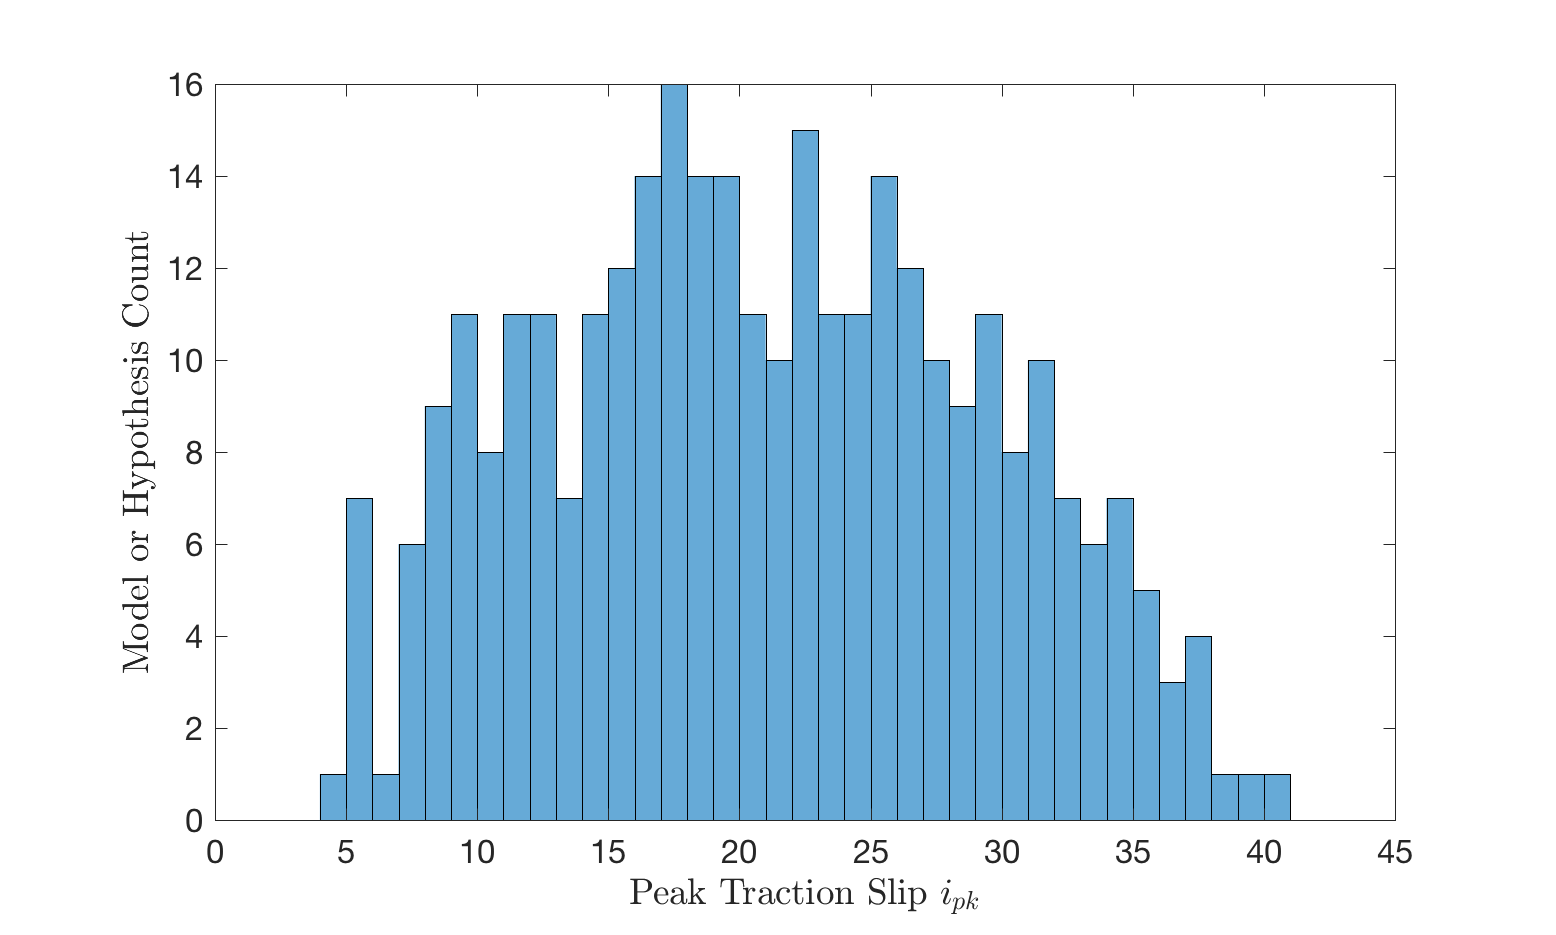
\includegraphics[width = 4in, keepaspectratio]{histogram_peak_slip}
    \caption{Histogram of the peak slip values $i_{pk}$ for generating the maximum net traction value $F_{net}$ for each of the models or hypotheses considered from section \ref{s:MME}}
    \label{fig:histogram_peak_slip}
\end{figure}
Since most of the terrain models have $i_{pk} \leq 25\%$ the traction control is entered once $\hat{i} > 25 \%$. Higher threshold values were experimented with but led to failure of the control mode since the controller turns on too late to prevent immobilzation. The slip threshold used for exiting the traction control mode is $\hat{i} < 5\%$. This is chosen since data collected in Antarctica in Fig. \ref{fig:Model_Validation_Plot_Sim} show slip values below this threshold on firm terrain and it is below almost all $i_{pk}$ values in Fig. \ref{fig:histogram_peak_slip}